\chapter{The process}
 
\label{cha:first_principles_model}
\todo[inline]{This is where the results are supposed to go, so there should be an introduction to them}
In regards to modelling, most of the work already been done in \cite{waste_prof}. \todo[inline]{It is possible to cite Stochastic Disturbances and Dynamics of Thermal Processes with application to municipal solid waste combustion. PhD thesis, Eindhoven University of Technology,}. As a result, there will only a quick summary of the process will be given in this thesis. The model does make some simplifications on the dynamics of the system, most notably when it comes to transport-delay. Those simplifications will be discussed in a later section \todo[inline]{Add the later section}


\section{Process overview}

\begin{figure}[htbp]
    \centering
    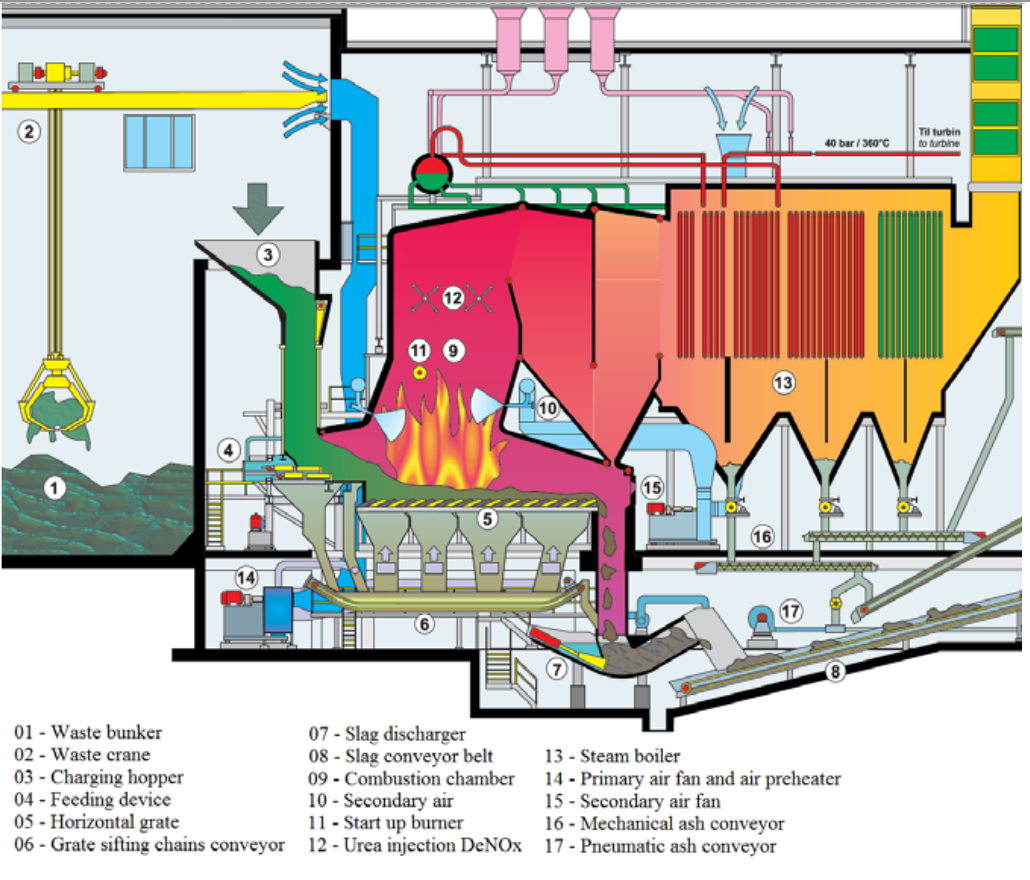
\includegraphics[width=\textwidth]{img/plant_overview.png}
    \caption{Overview of the plant}
    \label{fig:plant_overview}
  \end{figure}
  

As seen in Figure \ref{fig:plant_overview}, the waste is normally delivered to the waste-bunker (1). There, a set of cranes are used to mix it, in order to make it more homogeneous. Some of it is then fed into the charging hopper (3) by the same cranes. A ram (4) pushes the waste onto the waste-grates (5). While on the grate, the primary air-flow (17) dries the waste and provides oxygen for the primary combustion\todo[inline]{Find the difference between solid combustion and gaseous combustion}. The grates are divided into three sections. The waste is dried on the first section. On the second section of the grate, the primary combustion happens. On the third part of the grate, the post-combustion has to occur. This is to ensure that the amount of combustible material in the ash is below a certain threshold\footnote{In addition to the environmental damage that may come from exceeding these limits for too long, the limits are also enforced by law}. The ash is then removed(17) from the system to be cleaned and disposed of. The combustion also results in the production of heat and various gasses, which are added to the flue-gas. Somewhere above the second part of the grate, a secondary airflow is also applied to the volatile gases resulting from the primary combustion. This is where secondary combustion occurs. The primary and secondary airflow(10) provide oxygen to the fire so that the combustion is complete. The two airflows are needed because complete combustion will not occur unless the oxygen is added and mixed properly into the two combustion processes. This will only occur if the oxygen is added both through the primary and the secondary airflow, even if the stochiometry would have allowed for all the oxygen to be added at one point. The heat-exchange between the burning waste and the flue gas happens through contact, a mass-stream of gases from the combustion and by radiation. The flue gas in the combustion chamber(9) has a temperature of roughly $800^O C$ and is highly corrosive, so urea is added to the gas make it less reactive \todo[inline]{by removing what?} before it can be used to heat the boiler(13). The flue gas travels through multiple bends while giving off heat before reaching the heat exchange elements that are used to heat the boiler. The flue gas then reaches the heat-exchange elements, where it is used to heat the saturated steam that is connected to a drum. The water is under pressure, so it will usually be warmer than $100^\circ C$. Finally, the flue gas exits out of the system that is to be controlled in this thesis and into the part of the plant where it is cleaned before being released into the atmosphere. The composition of the flue gas that is released will depend on the amount of primary and secondary oxygen, the temperature in the combustion chamber, as well as the composition of the waste that is being burned. The cleaning systems used for removing the $NO_x$ from the flue gas are not very good at handling sudden spikes in concentration, so one of the primary objectives of the controller is to keep the concentration of oxygen above a certain threshold (Normally 6\%, sometimes 3.5\%)

\section{Quirks of the system}

Just like any system, there are non-linearities in a combustion process as well. Ideally, the relationship between the inputs and the outputs should be as linear as possible. Additionally, the actual objective of installing the plant is not the same as just making the control variables follow the reference, but rather to keep the concentration of $NO_x$ and similar unwanted bi-products to a minimum. For simplicity, it might be useful to take a look at the controller structure that has been used on the plant in previous instances. 

\begin{figure}
  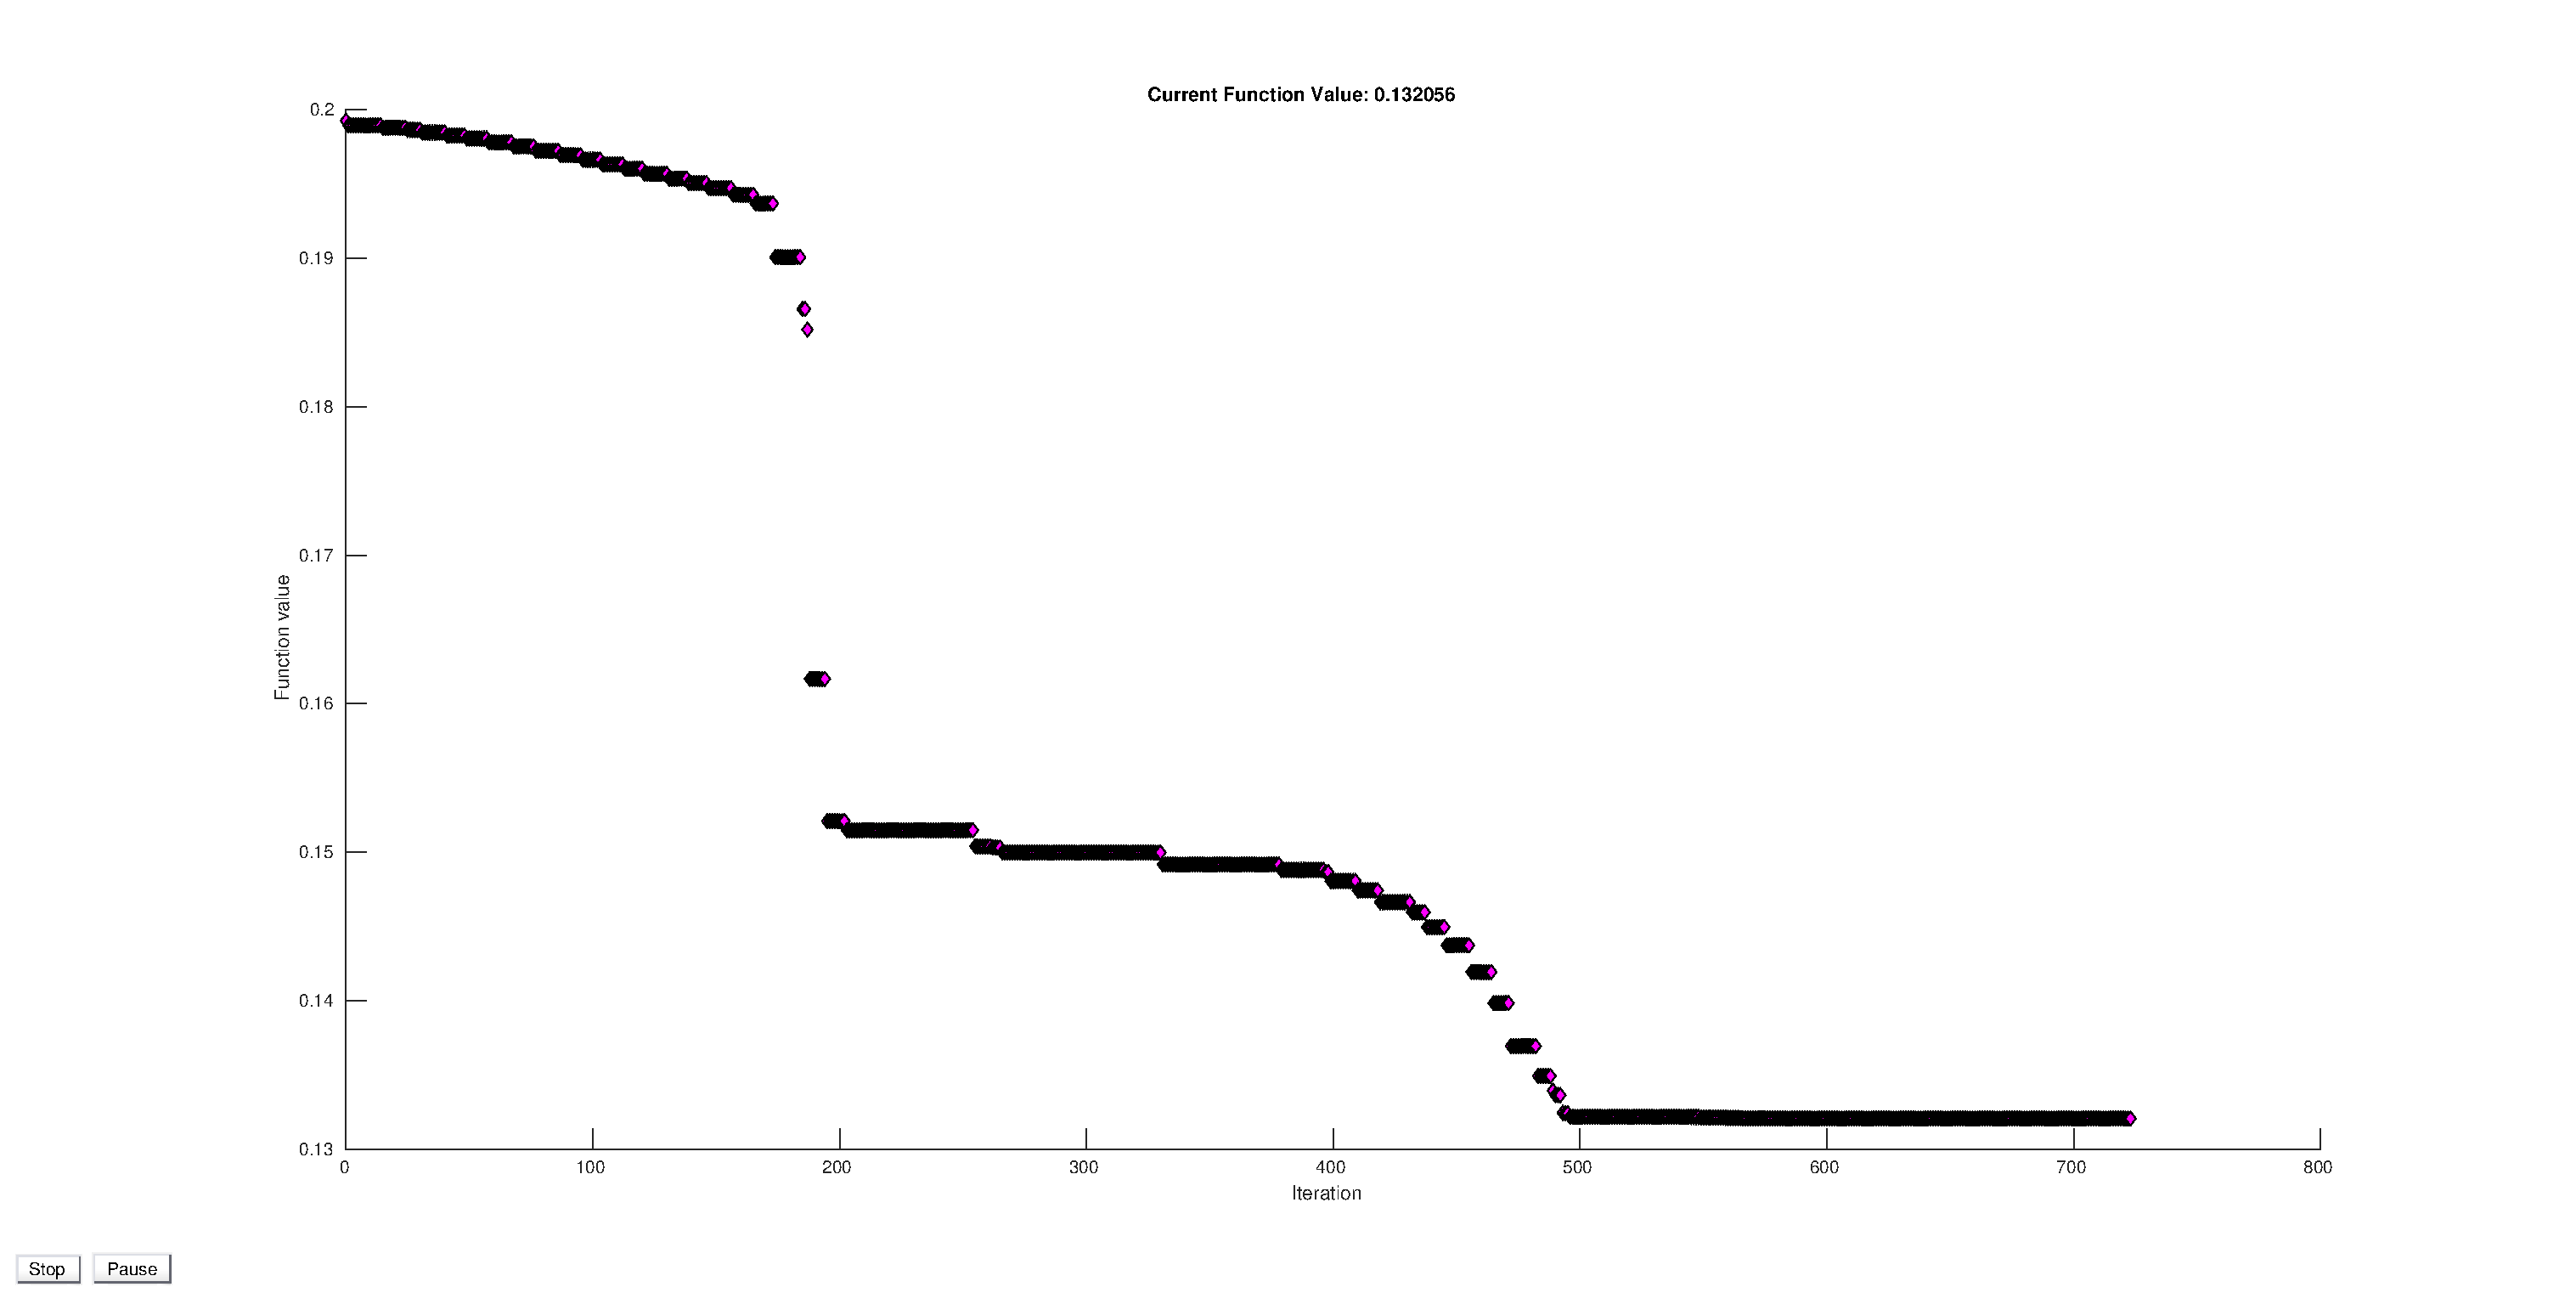
\includegraphics[width=\textwidth]{img/autotune_PID_progress.eps}
  \label{fig:AB_controller_structure}
  \caption{A/B-controller structure}
\end{figure}

\todo[inline]{Add a figure of the model structure here}
\noindent
The previous model expressed the plant as in \ref{fig:AB_controller_structure}. Here, the inputs were chosen to be primary air, secondary air, and grate-speed and ram speed. The outputs were chosen to be the mass flow of produced steam $F_{st}$, the mass flow of oxygen in the flue gas $F_{O2}$ and the ratio of primary air to secondary air. In the cascaded A/B-controller, an extra output $\hat{HHV}$ was added. This is the estimate of the heating value. $\hat{HHV}$ is estimated form a product between the mass-flow of flue gas, the heat capacity of each component and the difference in temperature between the ambient air and the temperature of the flue gas. This means that $\hat{HHV}$ is a measure power. If the temperature of the produced steam is constant, then $F_{st}$ also be proportional to some amount of power. The same goes for $F_{w,in}$, as long as the composition of the waste remains constant. The amount  of oxygen in the flue gas should be proportional to $F_{aII}$ and $F_{aI}$ while being negatively proportional to the amount of waste burned. So, as long as the distribution of heat between the flue gas and the ash is very dependent on the change in temperature, of if the heat-exchange with the outside world is very dependant on some non-linear characteristics, then there is reason to assume that the inputs and outputs have a somewhat linear relation. This is most notable since it probably leads to far better results than using temperature as one of the measures. 

\noindent
With the measurements that currently available in the plant, these are some of the best available candidates. Some alternatives to inputs and outputs is to use expected enthalpy as an input instead of simply using the waste-flow. Even though a similar guess could be made for the relationship between $F_{aI}$ and $F_{aII}$, this is not true, as seen in figure \ref{fig:compare_steam_by_air}. This is because the spike in steam production resulting from the secondary air ends quite a bit earlier than the other one. 

\begin{figure}
  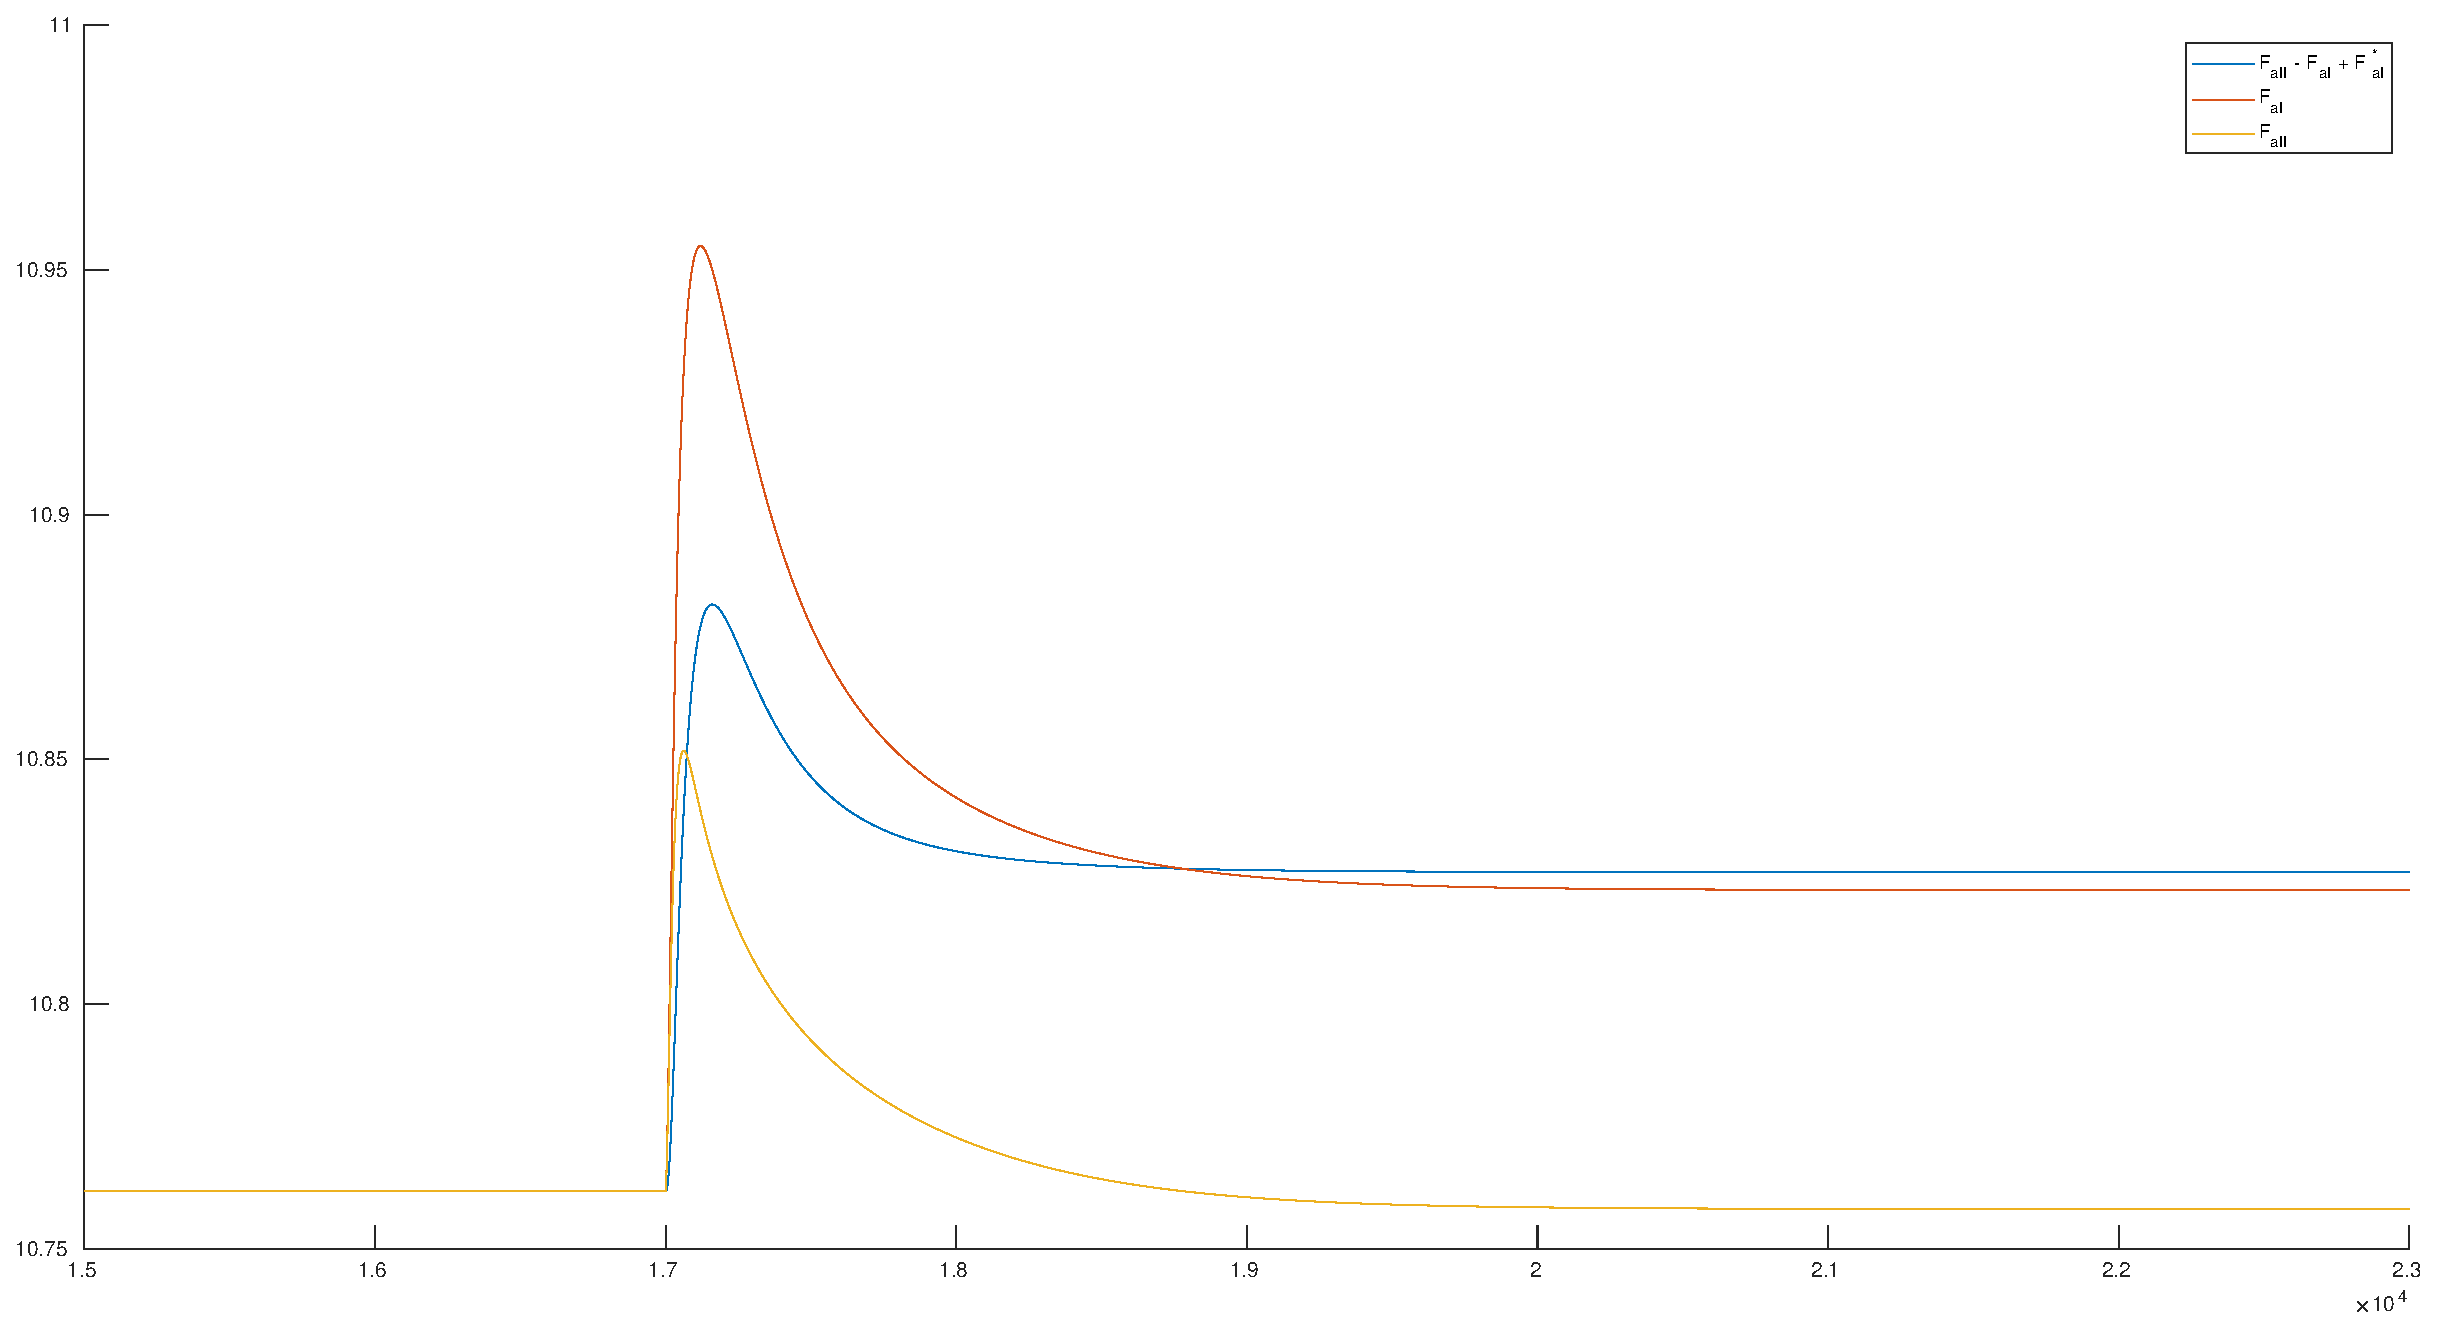
\includegraphics[width=\textwidth]{img/compare_steam_from_air_inputs.eps}
  \label{fig:compare_steam_by_air}
  \caption{Change in steam production as a result of changes in air}
\end{figure}
\noindent
Finally, and most importantly, the fact that the oxygen concentration and steam production remains constant is not in of itself the goal of the controller. If these two values remain constant, it usually means that the combustion within the furnace remains constant, which results in a low concentration of $NO_x$. But, as has already been noted, if the difference between the primary and the secondary air is too large, then the reactants in the combustion process don't get mixed properly, which will result in the production of $NO_x$, even if $F_{st}$ and $F_{O2}$ look good. As a result, it is also an objective to keep $\frac{F_{aI}}{F_{aII}}$ at a constant ratio. That is the reason for why one of the PIDs in the standard A/B-controller uses the ratio between primary air and secondary air for one of its error signals. 

\todo[inline]{Fill in about the nature of the parameters, and how power is proportional to waste-flow}
\todo[inline]{I left off here}
\todo[inline]{Formulate this part better (?)}

\todo[inline]{take a look at the possibilities for using enthalpy as an input, or delivered power as an output}